\begin{enumerate}
	\item
	\begin{enumerate}
		\item $\begin{gathered}\lim\limits_{\substack{x \to 0\\x>0}}f(x) = \lim\limits_{\substack{x \to 0\\x>0}}\left[5x^2 + 2x - 2x^2\ln(x)\right]\end{gathered}$
		
		\[\left.
		\begin{array}{r}
			\lim\limits_{x \to 0}\left(5x^2+2x\right) = 0\\
			\text{Par croissance comparée}\: \lim\limits_{\substack{x \to 0\\x>0}}x^2\ln(x) = 0
		\end{array}\right\} \overset{\substack{\text{par} \\ \text{somme}}}{\implies} \lim_{\substack{x \to 0\\x>0}}\left[5x^2 + 2x - 2x^2 \ln (x)\right] = 0\]
		
		\[\boxed{\lim_{\substack{x \to 0\\x>0}}f(x) = 0}\]
		\item $\lim\limits_{x \to +\infty}f(x) = \lim\limits_{x \to +\infty}\left[5x^2+2x-2x^2\ln (x)\right] = \lim\limits_{x \to +\infty}x^2\left[5+\dfrac{2}{x}-2\ln(x)\right]$
		
		\[\renewcommand{\arraystretch}{2}
		\left.
		\begin{array}{r}
			\lim\limits_{x \to +\infty}\dfrac{2}{x} = 0 \implies \lim\limits_{x \to +\infty}\left(5+\dfrac{2}{x}\right) = 5 \\
			\lim\limits_{x \to +\infty}\ln(x) = +\infty \implies \lim\limits_{x \to +\infty}-2\ln(x) = -\infty
		\end{array}\right\} \overset{\substack{\text{par} \\ \text{somme}}}{\implies} \lim_{x \to +\infty}\left[5 + \dfrac{2}{x} - 2\ln (x)\right] = -\infty
		\]
		
		\[\renewcommand{\arraystretch}{2}
		\left.
		\begin{array}{r}
			\lim\limits_{x \to +\infty}x^2 = +\infty \\
			\lim\limits_{x \to +\infty}\left[5 + \dfrac{2}{x} - 2\ln (x)\right] = -\infty
		\end{array}\right\} \overset{\substack{\text{par} \\ \text{produit}}}{\implies} \lim_{x \to +\infty}x^2\left[5+\dfrac{2}{x}-2\ln(x)\right] = -\infty
		\]
		
		\[\boxed{\lim_{x \to +\infty}f(x) = -\infty}\]
	\end{enumerate}
	\item\
	\begin{eqnarray*}
		f'(x) &=& 5 \times 2x + 2 - 2 \left[ 2x \times \ln(x) + x^2 \times \dfrac{1}{x}\right] = 10x + 2 - 2\left[2x\ln(x) + x\right] = 10x + 2 - 4x\ln(x) - 2x\\
		&=& \boxed{8x + 2 - 4x\ln(x)}
	\end{eqnarray*}
	\item
	\begin{enumerate}
		\item
		\[f''(x) = 8 - 4\left[1 \times \ln(x) + x \times \dfrac{1}{x}\right] = 8 - 4\ln (x) - 4 = 4 - 4\ln(x) = \boxed{4\left[1-\ln(x)\right]}\]
		\item La courbe $\mathcal{C}_f$ est au-dessus de ses tangentes si, et seulement si, $f$ est convexe, ce qui équivaut à $f''(x)$ est positif.
		
		$f''(x) \geqslant 0 \iff 4\left[1-\ln(x)\right] \geqslant 0 \iff 1-\ln(x) \geqslant 0 \iff -\ln(x) \geqslant -1 \iff \ln(x) \leqslant 1 \iff x \leqslant \text{e}$ (car la fonction ln est strictement croissante sur $]0~;~+\infty[$).\\
		\smallskip
		
		La courbe $\mathcal{C}_f$ est donc au-dessus de ses tangentes sur l'intervalle $]0~;~\text{e}]$.
		\item\
		\begin{center}
		\begin{tikzpicture}
		\tkzTabInit[lgt=2.5,espcl=3]{$x$/1,Signe de $f''(x)$/1,Variations de $f'$/2.5}{$0$,e,$+\infty$}
		\tkzTabLine{d,+,z,-,}
		\tkzTabVar{D-/$2$,+/$4\text{e}+2$,-/$-\infty$}
		\end{tikzpicture}
		
		$f'(\text{e}) = 8\text{e} + 2 - 4\text{e} \ln(\text{e}) = 8\text{e} + 2 - 4\text{e} = 4\text{e} + 2$
		\end{center}
	\end{enumerate}
	\item
	\begin{enumerate}
		\item Sur $]0~;~\text{e}]$, la fonction $f'$ est strictement croissante avec $\begin{gathered}\lim\limits_{\substack{x \to 0\\x>0}}f'(x) = 2\end{gathered}$, donc pour tout $x \in ]0~;~\text{e}]$,on a $f'(x) > 0$.\\
		\smallskip
		
		Sur $[\text{e}~;~+\infty[$, la fonction $f'$ est continue (puisque dérivable) et strictement décroissante. De plus, $f(_text{e}) = 4\text{e} + 2 > 0$ et $\lim\limits_{x \to +\infty}f'(x) = -\infty$. $0 \in ]-\infty~;~4\text{e}+2[$, donc, d'après le corollaire du théorème des valeurs intermédiaires, l'équation $f'(x) = 0$ admet une solution unique $\alpha$ sur $[\text{e}~;~+\infty[$.\\
		\smallskip
		
		Au final, l'équation $f'(x) = 0$ admet une solution unique $\alpha$ sur $]0~;~+\infty[$.\\
		\medskip
		
		On a :
		\[\boxed{\np{7.87} < \alpha < \np{7.88}}\]
		\item On sait que sur $]0~;~\text{e}]$ on a $f'(x) > 0$. Puisque $f'$ est décroissante sur $[\text{e}~;~+\infty[$ et qu'elle s'annule en $\alpha$, $f'(x) \geqslant 0$ sur $[\text{e}~;~\alpha]$ et $f'(x) \leqslant 0$ sur $[\alpha~;~+\infty[$. Donc $f'(x)$ est positif sur $]0~;~\alpha]$ et négatif sur $[\alpha~;~+\infty[$.
		
		\begin{center}
		\begin{tikzpicture}
		\tkzTabInit[lgt=2.5,espcl=3]{$x$/1,Signe de $f'(x)$/1,Variations de $f$/2.5}{$0$,$\alpha$,$+\infty$}
		\tkzTabLine{d,+,z,-,}
		\tkzTabVar{D-/$0$,+/$f(\alpha)$,-/$-\infty$}
		\end{tikzpicture}
		\end{center}
	\end{enumerate}
	\item On a $f''(\alpha) = 8\alpha + 2 - 4\alpha \ln(\alpha)$, donc :
	\begin{eqnarray*}
		f'(\alpha) = 0 &\iff& 8\alpha + 2 - 4 \alpha \ln(\alpha) = 0\\
		&\iff& 4\alpha\ln(\alpha) = 8\alpha + 2\\
		&\iff& \ln(\alpha) = \dfrac{2(4\alpha+1)}{4\alpha} \qquad (\alpha \neq 0)\\
		&\iff& \boxed{\ln(\alpha) = \dfrac{4\alpha+1}{2\alpha}}
	\end{eqnarray*}
	
	On a donc :
	\begin{eqnarray*}
		f(\alpha) &=& 5\alpha^2 + 2\alpha - 2\alpha^2 \ln(\alpha) \\
		&=& 5\alpha^2 + 2\alpha - 2\alpha^2 \times \dfrac{4\alpha+1}{2\alpha} \\
		&=& 5\alpha^2 + 2\alpha - \alpha(4\alpha + 1) \\
		&=& 5\alpha^2 + 2\alpha - 4\alpha^2 - \alpha \\
		&=& \boxed{\alpha^2  + \alpha}
	\end{eqnarray*}
	\item D'après la question \textbf{4.a.}, on a :
	\begin{eqnarray*}
		\np{7.87} < \alpha < \np{7.88} &\iff& \np{61.9369} < \alpha^2 < \np{62.0944} \\
		&\iff& \np{69.8069} < \alpha^2 + \alpha < \np{69.9744} \\
		&\iff& \boxed{\np{69.8069} < f(\alpha) < \np{69.9744}}
	\end{eqnarray*}
\end{enumerate}
